%========================================
% Comp2129
%========================================

\documentclass[10pt, multicolumn, a4paper]{article}

\usepackage{amsmath} % just math
\usepackage{amssymb} % allow blackboard bold (aka N,R,Q sets)
\usepackage{ulem}
\usepackage{enumitem}
\usepackage{tikz}
\setlist{nolistsep}
\usepackage{multicol}
\linespread{1.6}  % double spaces lines
\usepackage[left=1in,top=1in,right=1in,bottom=1in,nohead]{geometry}

\begin{document}

\linespread{1} % single spaces lines
\small \normalsize %% dumb, but have to do this for the prev to work
%\begin{flushright}
%Comp2129
%\end{flushright}

% http://linux.die.net/man/2/getrusage
% get a process's resource usage, such as elapsed time, from inside the process

%========================================
% Lecture 2
%========================================

\setcounter{section}{1} % first section is now 2
\hrule
\section{Introduction to C} 
\hrule

\begin{multicols}{2}
	\subsection*{C Modules}
	\begin{itemize}
	\item file translated into obj. file, which gets linked by linker to other object files and std libraries
	\item can refer to global variables/functions of other modules via. externs
	\end{itemize}
	\subsection*{Char input/output}
	\begin{itemize}
	\item \verb|getchar(void)|
	\item \verb|putchar(c)|
	\end{itemize}
	\subsection*{\texttt{printf()} string formats}
	\begin{itemize}
	\item \verb|%.2f| floating pt to 2dp
	\item \verb|%p| pointer
	\end{itemize}
	\subsection*{\texttt{scanf()}}
	\begin{itemize}
	\item reads from std input
	\item returns number of read items
	\item parameters must be pointers
	\end{itemize} 
\end{multicols}

\setcounter{section}{1} % first section is now 2
\hrule
\section{Introduction to Unix}
\hrule 

\begin{multicols}{2}
	\subsection*{\texttt{file}}
	\begin{itemize}
	\item determines type of file
	\item e.g. ordinary, directory, device, 'special'
	\end{itemize}
	\subsection*{Shell environment}
	\begin{itemize}
	\item at login, reads from \verb|/etc/profile|
	\item gets \verb|.bash_profile|, \verb|.profile|
	\end{itemize}
	\subsection*{Permissions}
	\begin{itemize}
	\item user, group, other
	\item read, write, execute
	\item use magical numbers (r: 4, w: 2, x: 1)
	\end{itemize}
	\subsection*{Redirections}
	\begin{itemize}
	\item \verb|a.out < data >res 2>errors|
	\item appending: \verb|>>|
	\end{itemize}
	%\subsection*{Pipes}
	%\begin{itemize}
	%\item takes output from last cmd and uses it as input for the next
	%\end{itemize}
	\subsection*{Shell scripts}
	\begin{itemize}
	\item \verb|#!/bin/bash|
	\item default search path \verb|$PATH|
	\item to execute a script, \verb|./scriptname|, otherwise if the current dir is in \verb|$PATH| it can be executed using \verb|scriptname|
	\end{itemize}
	\subsection*{Shell}
	\begin{itemize}
	\item UNIX cmd interpreter
	\item reads in cmds, runs appropriate programs
	\end{itemize}
	\subsection*{I/O redirection}
	\begin{itemize}
	\item when prog runs, 3 std files opened 
		\\ \verb|0| std input \\ \verb|1| std output \\ \verb|2| std error
	\end{itemize}
	\subsection*{Shell variables}
	\begin{itemize}
	\item stored in environment of the program
	\item setting: \verb|VARNAME=value|
	\item using: \verb|$VARNAME|
	\item script arguments: \verb|$1, $2| etc.
	\end{itemize}
	\subsection*{\texttt{if} statement}
	\begin{itemize}
	\item \texttt{if <cmd> \\ then \\ \hspace*{5mm} <cmd> \\ fi}
	\end{itemize}
	\subsection*{\texttt{while} loop}
	\begin{itemize}
	\item \texttt{while <condition> \\ do \\ \hspace*{5mm} <cmd> \\ done}
	\end{itemize}
	\subsection*{\texttt{for} loop}
	\begin{itemize}
	\item \texttt{for <condition> \\ do \\ \hspace*{5mm} <cmd> \\ done}
	\end{itemize}
	\subsection*{\texttt{case}}
	\begin{itemize}
	\item \texttt{case \$selector in \\ 1) <cmd> ;; \\ 2) <cmd> ;; \\ esac}
	\end{itemize}
	\subsection*{UNIX cmds}
	\begin{itemize}
	\item \texttt{test}: tests a condition, exists with true/false
		\\ \texttt{if test \$1 == "blah"}
	\item \texttt{sort}: sorts lines of text in a file
	\item \texttt{cut}: cuts selected parts of lines of text in a file, and sends result to output
	\item \texttt{tr}: changes or removes chars from a file
	\item \texttt{comm}: compares files and prints lines that exist in only one or both files
	\item \texttt{grep}: searches text file/output, matching each line against specified regex, and prints all lines that match
	\item \verb|diff| and \verb|sdiff|: comparing files
	\end{itemize}
	\subsection*{Cmd substitution}
	\begin{itemize}
	\item arg enclosed in backquotes indicates that a command is to run, and the output used as the actual argument(s)
	\item \verb|prog `cat argfile`|
	% $(command) which is like `command`, but you can nest them correctly: $(command $(command2)) which you can't do with backticks ` `
	\end{itemize}
	\subsection*{Subshells}
	\begin{itemize}
	\item run cmds in another copy of the shell
	\item environment copied from parent - subshell can change environ., but it will be reverted when the subshell exits
	\item \texttt{tar cf – mydir | (cd *loc*; tar xf -)}
	\end{itemize}
	\subsection*{Collecting output}
	\begin{itemize}
	\item \verb| (echo data; cat filename) > output|
	\end{itemize}
	\subsection*{Arithmetic}
	\begin{itemize}
	\item \verb|expr| evaluates its args as an expression
	\item \verb|let| for assignment of variables 
	\item \verb|let “count = count +1”|
	\end{itemize}
	\subsection*{Read text from shell}
	\begin{itemize}
	\item \verb|read x|: reads in line from std input, and stores as x
	\item "here document"
	\end{itemize}
	\subsection*{Finding files}
	\begin{itemize}
	\item \verb|find|: starts at curr dir and searches recursively
	\item \verb|locate|: prints the full path names of all files that match
	\item \verb|du|: prints disk usage starting at curr dir
	\end{itemize}
	\subsection*{Strange file names}
	\begin{itemize}
	\item to open file named \verb|-x|, use \verb|nano ./-x|
	\item \verb|--| to stop parsing flags \\ \verb|rm -- -x|
	\end{itemize}
	% SDNT: For shits and gigs go through web generation example
\end{multicols}

%========================================
% Lecture 3
%========================================

\hrule
\section{Pointers}
\hrule 

\begin{multicols}{2}
	\begin{itemize}
	\item a memory address
	\item obtain address of variable with \verb|&|
	\item create pointer to the address of \verb|initial| \\
		\verb|char initial = 'A';| \\ \verb|char *initial_ptr = &initial;|
	\item \verb|*| pointer to variable of specific type
	\item \verb|**| unravels indirection
	\item \verb|char msg[] = "message";| \\ \verb|char *string = &msg[0];| (or \verb|msg|)
		\\ $\therefore$ \verb|msg[1] == *(string+1)|
	\item Iterating through a string with a pointer
		\\ \verb|while (*str != '\0') { str++; }|
	\end{itemize}
	\subsection*{Dynamic data structures}
	\begin{itemize}
	\item dynamically allocate memory
	\item \verb|malloc|, \verb|realloc| etc.
	\end{itemize}
	\subsection*{Indirection operator}
	\begin{itemize}
	\item declaration: pointer to specified type \\ \verb|int * ptr|
	\item dereferencing: dereferences the pointer to mean the content/value of the variable being pointed to
	\end{itemize}
	\subsection*{Array processing}
	\begin{itemize}
	\item \verb|int array[10]| \\ \verb|array == &array[0]|
	\item variables can change their values, but not their addresses
	\item pointer's value is the address of another variable, $\therefore$ arithmetic ops permitted on pointer
	% SDNT: Squiz this more pls
	\end{itemize}
	\subsection*{Pointer scalars}
	\begin{itemize}
	\item mathematical operations on pointers work regardless of the data type being pointed to
	\item ptr accesses to arrays will always move the correct number of bytes
	\end{itemize}
	\subsection*{Pass by reference}
	\begin{itemize}
	\item swaps addresses of initial variables
	\item \verb|void swap (int *a, int *b) {| \\ \texttt{\hspace*{5mm} int tmp = *a; \\ \hspace*{5mm}  *a = *b; \\ \hspace*{5mm} *b = tmp;} \\ \verb|}|
	\end{itemize}
	\subsection*{Pointers to pointers}
	\begin{itemize}
	\item multiple indirection
	\item \verb|argv[][] == *argv[] == **argv|
	\end{itemize}
	\subsection*{\texttt{void} pointers}
	\begin{itemize}
	%\item no associated scalar value
	\item type signature of the pointer does not specify what it's pointing to
	% that doesn't mean it doesn't have an "associated scalar value", it just means that the type signature doesn't indicate the type of the value, you can still interpret it as a pointer to any type you like
	\item can recieve/return ptrs of any type
	\item \verb|void *malloc(size_t size);|
	\end{itemize}
	\subsection*{Function pointers}
	\begin{itemize}
	\item refer to 12. string handling
	\item allows for selection of program behavior
	\end{itemize}
	\subsection*{\texttt{NULL} pointers}
	\begin{itemize}
	\item pointer to something at address '0'
	\item invalid to read or write to that address $\therefore$ god
	%\item denotes invalid pointer, not a ptr to something at address '0'
	%it's a pointer to something at address 0, it's just usually invalid to read or write to that address, so it's used as a "sentinel", without ever being dereferenced
	\end{itemize}
\end{multicols}

\setcounter{section}{2}
\hrule
\section{Aggregate Data Structures}
\hrule 

\begin{multicols}{2}
	\subsection*{enums}
	\begin{itemize}
	\item associates name to a value
	\item maps to an int
	\item \verb|enum day_name {| \\ \texttt{\hspace*{5mm} mon, tue, wed, thur, fri, sat, sun} \\ \verb|}|
		\\ maps to ints 0..7
	\item can then use \verb|sun++;|
	\end{itemize}
	\subsection*{Structures}
	\begin{itemize}
	\item for a collection of data items of different types
	\item \verb|struct <tag> {|	\\ \texttt{\hspace*{5mm} <member-declarations>} \\ \verb|}|
	\item declare: \verb|struct <tag> <identifier-list>;|
	\item access: \verb|<identifier>.<element>;|
	\item if a pointer to a struct is used, \verb|->| operator is used to get an element in a struct
	\end{itemize}
\end{multicols}

%========================================
% Lecture 4
%========================================

\hrule
\section{Source Code Control}
\hrule 

\begin{multicols}{2}
	\subsection*{Issues}
	\begin{itemize}
	\item version control
	\item managing several versions of a program
	\item allows you to maintain current version whilst working on the next
	\end{itemize}
	\subsection*{Control}
	\begin{itemize}
	\item checkin/checkout system
	\item e.g. svn, git, hg
	\end{itemize}
	\subsection*{Mercurial: hg}
	\begin{itemize}
	%\item works in own directory
	%\item keeps versions of your code
	%\item allows you to revert to older versions
	%\item changeset records: author, descrip., what changes were, what files changed etc.
	\item distributed
		\begin{enumerate}
		\item make copy of existing repo
		\item push changes to others
		\item pull changes from others
		\end{enumerate}
	\item \verb|hg init|: creates repo
	%\item \verb|hg add code.c|: add file code.c to repo
	%\item \verb|hg diff|: diff between curr and prev version
	\item \verb|hg diff -r2 -r3|: diff b/w revision 2 and 3
	\item \verb|hg revert -r2 code.c|: revert file to r2
	\item \verb|hg push/pull/clone <repo>|
	\item repo: another dir/URL to a remote repo
	%\item merges unless there are conflicts, which are reported and can be fixed manually
	\end{itemize}
\end{multicols}

\setcounter{section}{3}
\hrule
\section{\texttt{make}}
\hrule 

\begin{multicols}{2}
	\begin{itemize}
	\item program can use many \verb|.c|, \verb|.h| files that require compiling
	\item time consuming to compile lots of files separately
	\item object file: machine language, but not yet linked with other parts of the program
	\item several \verb|.c|,  \verb|.o| files can be combined to give an executable program via. linkage
	\item after changing one \verb|.c| file, you need to recompile affected file and relink $\therefore$ \verb|make| is sexy
	\end{itemize}
	\subsection*{Rules}
	\begin{itemize}
	\item \verb|prog.o: prog.c prog.h| \hspace*{5mm} dependencies 
		\\ \texttt{\hspace*{5mm} gcc -c prog.c} \hspace*{13mm} action
	\item \verb|<target>|: name of file to be made
	\item \verb|<1+ dependencies>|%: files the target file depends on
	\item \verb|<action>|: shell cmd that creates target
	\item default rules are the bomb
	\item can combine rules when targets have common dependencies and actions
	\item can create rules without dependences
		\\ \verb|clean:| \\ \texttt{\hspace*{5mm} rm *o}
	\end{itemize}
	
	\newpage	
	
	\subsection*{\texttt{make} variables}
	\begin{itemize}
	\item assignments: \verb|variable_name = value|
	\item use: \verb|$(variable_name)|
	\end{itemize}
	\subsection*{Predefined variables}
	\begin{itemize}
	\item \verb|CC|: default C compiler
	\item \verb|CFLAGS|: flags passed to the C compiler
	\end{itemize}
	\subsection*{Libraries}
	\begin{itemize}
	\item gives you the ability to store the object code versions of the functions in one place and have them linked into your program
	\item stdlib automatically searched when prog is linked
	\item use functions from other libraries using \verb|-l| flag when linking
	\item the C compiler will search for the library in standard directories: \verb|/lib, /usr/lib|
	\item create own library using \verb|ar|, which makes library mylib.a and will contain specified .o files
		\\ \verb|ar c mylib.a readit.o util.o|
	\item can then use created library when compiling
		\\ \verb|gcc myprog.o mylib.a -o myprog|
	\end{itemize}
\end{multicols}

%========================================
% Lecture 5
%========================================

\hrule
\section{Memory Management}
\hrule 

\begin{multicols}{2}
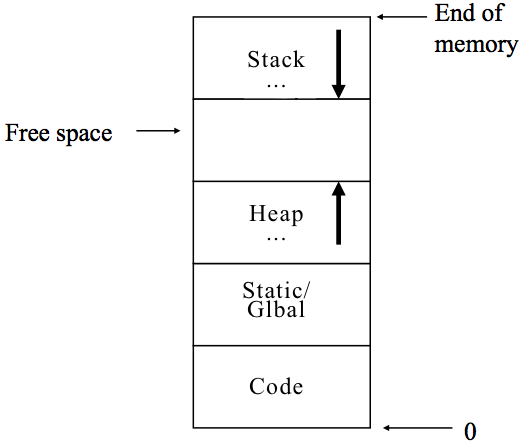
\includegraphics[scale=.6]{mem_management.png}
	\subsection*{Memory areas}
	\begin{itemize}
	\item code: program instructions
	\item global/static: global/static variables
	\item stack: local variables, function arguments, return addresses, temporary storage
	\item heap: dynamically allocated memory
	\end{itemize}
	\subsection*{Stack}
	\begin{itemize}
	\item all variables local to a function and function args stored on the stack
	\item to call func:
		\begin{enumerate}
		\item push args to stack
		\item push return address to stack
		\item jump to function code
		\end{enumerate}
	\item inside function:
		\begin{enumerate}
		\item increment the stack pointer to allow space for the local variables
		\item execute the code
		\item pop local variables and arguments off the stack 
		\item push the return result onto the stack
		\item jump to return address
		\end{enumerate}
	\end{itemize}
	\subsection*{Heap}
	\begin{itemize}
	\item accessed under direct control
	\item request allocation, if there is sufficient contiguous memory available, a pointer is returned to the address of the stage of that memory block
	\end{itemize}
	\subsection*{Memory allocation functions}
	\begin{itemize}
	\item returns a pointer to void 
	\item pointer must be cast to a specific type
	\end{itemize}
	\subsection*{\texttt{malloc}}
	\begin{itemize}
	\item \verb|void *malloc(size_t size)|
	\item requests number of bytes of memory
	\end{itemize}
	\subsection*{\texttt{calloc}}
	\begin{itemize}
	\item \verb|void *calloc(size_t num, size_t size)|
	\item requests number of blocks of memory, and the size of each block
	\item allocated memory is cleared i.e. set to '0'
	\end{itemize}
	\subsection*{\texttt{realloc}}
	\begin{itemize}
	\item \verb|void *realloc(void *ptr, size_t size)|
	\item takes previously allocated memory, and attempts to resize it
	\item contents are preserved
	\item may require new block of memory (for contiguous-ness) $\therefore$ new void pointer is returned
	\end{itemize}
	\subsection*{\texttt{free}}
	\begin{itemize}
	\item \verb|void free(void *ptr)|
	\item deallocates memory previously allocated 
	\item \verb|valgrind|: check for leaks
	\end{itemize}
	\subsection*{to make program happy}
	\begin{itemize}
	\item check memory allocation for success (NULL pointer is returned if unsuccessful)
	\item don't free memory that has already been freed or was never allocated
	\end{itemize}
\end{multicols}

\setcounter{section}{4}
\hrule
\section{Preprocessor}
\hrule 

\begin{multicols}{2}
	\begin{itemize}
	\item \verb|#include "decs.h"| $>$ copying declarations into every file
	\item useful for externs, tyedefs, struct definitions
	\end{itemize}
	\subsection*{Defined symbols}
	\begin{itemize}
	\item replace identifier with string, everywhere it appears in the program
	\item can be any string of characters, $\therefore$ should bracket arithmetic expressions
	\end{itemize}
	\subsection*{Macros}
	\begin{itemize}
	\item \verb|define min(a,b) ((a) < (b) ? (a) : (b))|
	\end{itemize}
	\subsection*{Conditional inclusion}
	\begin{itemize}
	\item \verb|#ifdef|, \verb|#ifndef|, \verb|#undef|
	\item \verb|#if|, \verb|#elif|, \verb|#else|, \verb|#end|
	\end{itemize}
	\subsection*{Predefined symbols}
	\begin{itemize}
	\item \verb|__LINE__|: current line number at any point
	\item \verb|__FILE__|: name of current program file
	\end{itemize}
	\subsection*{Preprocessor ninjaness}
	\begin{itemize}
	\item \verb|gcc -E| runs only preprocessor
	\item exploit \verb|#define| call by name, and \verb|#ifdef| etc. for conditional generation of hacky templates
	\end{itemize}
	
\end{multicols}

%========================================
% Lecture 6
%========================================

\hrule
\section{Unions and Bitfields}
\hrule 

\begin{multicols}{2}
	\subsection*{Unions}
	\begin{itemize}
	\item variables that occupy the same space
	\item \verb|union {| 
		\\ \hspace*{5mm} \verb|struct {| \\ \hspace*{10mm} \verb|/* struct guts */| \\ \hspace*{5mm} \verb|} type_one;|
		\\ \hspace*{5mm} \verb|struct {| \\ \hspace*{10mm} \verb|/* struct guts */| \\ \hspace*{5mm} \verb|} type_two;|
		\\ \verb|} info;|
	\item access elements: \verb|union_name.part_name|
	\item don't know which variant of the union is being used, $\therefore$ need to use a separate variable to indicate this
	\item \verb|struct catalog x;|
		\\ \verb|switch (x.holding_type) {| 
			\\ \hspace*{5mm} \verb|case book:| \\ \texttt{\hspace*{10mm} <do stuff> \\ \hspace*{10mm} break;}
			\\ \hspace*{5mm} \verb|case film:| \\ \texttt{\hspace*{10mm} <do stuff> \\ \hspace*{10mm} break;}
			\\ \verb|}|
	\end{itemize}
	
	\subsection*{Bitfields}
	\begin{itemize}
	\item can specify the size of bits for each element in a structure
	\item size placed after field name, with a colon
	\item \verb|struct IOdev {| \\
		\texttt{\hspace*{5mm} unsigned RW: 1; \\ \hspace*{5mm} unsigned Dirn: 8; \\
		\hspace*{5mm} unsigned mode: 3; \\ \hspace*{5mm} unsigned pad: 4;} \\ \verb|}|
	\item may not be portable:
		\begin{itemize}
		\item depends on compiler whether structs are padded
		\item endianness: whether fields are stored MSB or LSB
		\end{itemize}
	\item unpack bitfields from data: 
		\begin{itemize}
		\item don't need C bitfield syntax
		\item shift \verb|<< >>| and logical operators \verb|&| \texttt{ $\sim$ $\wedge$ |}
		\item \verb|R_W = x >> 15;|
		\item \verb|Dirn = (x >>7) & 0xFF;|
		\end{itemize}
	\end{itemize}

\end{multicols}

\setcounter{section}{5}
\hrule
\section{Linked Lists}
\hrule 

\begin{multicols}{2}
	%\begin{itemize}
	%\item dynamic $\therefore$ must allocate memory
	%\item have pointers to where next element of the list is located
	%\end{itemize}
	\subsection*{Internals}
	\begin{itemize}
	\item terminated by the NULL pointer
	\item have pointer to the first element
	\item don't lose your nodes, that'd be awkward
	\end{itemize}
	\subsection*{Characteristics}
	\begin{itemize}
	\item altering nth element:
		\begin{itemize}
		\item array: O(1)
		\item linked list: O(n)
		\end{itemize}
	%\item flexible structure
	%\item dynamic
	\end{itemize}
\end{multicols}

%========================================
% Lecture 7
%========================================

\hrule
\section{Parallelism}
\hrule 

\begin{multicols}{2}
	\subsection*{Origin}
	\begin{itemize}
	%\item no more performance gains for sequential 
	\item require continuous/reasonable performance improvements to support growing architecture
	\item portability, malleability, maintaining
	\end{itemize}
	
	\subsection*{Moore's Law}
	\begin{itemize}
	\item number of transistors that can be placed on a circuit is doubling approximately every 2 years
	\item bottlenecks: power density, wire delays, DRAM access latency
	\end{itemize}
	\subsection*{Hardware/software development}
	\begin{itemize}
	\item historically, transistors used to boost performance
	\item now, more cores per chip, $\therefore$ more, not faster processors
	\item can't find solution to obtain substantial performance improvement of single core CPUs
	\item require new parallel architecture
	\end{itemize}
	
	\subsection*{Task parallelism}
	\begin{itemize}
	\item processing the task in parallel
	\item dependencies between tasks - some must be processed before other tasks can occur
	\item task dependency graph \\ e.g. directed acrylic graph (DAG)
	\end{itemize}
	\usetikzlibrary{automata,positioning}
	\begin{tikzpicture}[shorten >=1pt,node distance=1.5cm,on grid,auto]
	\node[state] (t_1)   {$t_1$};
	\node[state] (t_2) [below=of t_1] {$t_2$}; 
	\node[state] (t_3) [below right=of t_1] {$t_3$}; 
	\node[state] (t_4) [below right=of t_2] {$t_4$}; 
		\path[->]
		(t_1) edge (t_2)
		(t_3) edge (t_4)
		(t_2) edge (t_4);
	\end{tikzpicture}
	
	\subsection*{Data parallelism}
	\begin{itemize}
	\item parallel work on the data of a task
	\item i.e. performing the same task to different data items at the same time
	\end{itemize}
	\subsection*{Task}
	\begin{itemize}
	\item computation that consists of a sequence of instructions
	\item a distinct part of programs/algorithms, as they can be decomposed into tasks
	\end{itemize}	
	
	\subsection*{Dependencies}
	\begin{itemize}
	\item execution order between 2 tasks
	\item no dependencies = maximum parallelism
	\begin{tikzpicture}[shorten >=1pt,node distance=1.5cm,on grid,auto]
	\node[state] (t_1)   {$t_1$};
	\node[state] (t_2) [below right=of t_1] {$t_2$}; 
	\node[state] (t_3) [above right=of t_2] {$t_3$}; 
	\node[state] (t_4) [below right=of t_3] {$t_4$};
	\end{tikzpicture}
	\item dependencies \\
	\begin{tikzpicture}[shorten >=1pt,node distance=1.5cm,on grid,auto]
	\node[state] (t_1)   {$t_1$};
	\node[state] (t_2) [below left=of t_1] {$t_2$}; 
	\node[state] (t_3) [below right=of t_1] {$t_3$}; 
	\node[state] (t_4) [below=of t_3] {$t_4$};
		\path[->]
		(t_1) edge (t_2)
		(t_1) edge (t_3)
		(t_2) edge (t_3)
		(t_3) edge (t_4);	
	\end{tikzpicture}
	\item impose partial ordering on tasks
	\item dependency is transitive
		\begin{itemize}
		\item if Ta $\rightarrow$ Tb and Tb $\rightarrow$ Tc, \\then Ta $\rightarrow$ Tc
		\end{itemize}
	\end{itemize}
	
	\subsection*{Stream programs}
	\begin{itemize}
	\item some programs work on streams of data (audio, video etc.)
	%\item split divides stream, join merges
	\item used for regular, repeating computations
	\item pipeline parallelism:
		\begin{itemize}
		\item pipeline: sequence of actors
		\item reads input from upstream data channel, outputs to downstream channel
		\item producer-consumer relationship (have dependencies)
		\item stateful actors can be parallelised \\
		\begin{tikzpicture}[shorten >=1pt,node distance=1.5cm,on grid,auto]
		\node[state] (t_1)  {$t_1$};
		\node[state] (t_2) [right=of t_1] {$t_2$};
		\node[state] (t_3) [right=of t_2] {$t_3$};
		\coordinate[right of=t_3] (d1);
		\coordinate[left of=t_1] (d2);
			\path[->]
			(t_1) edge (t_2)
			(t_2) edge (t_3);
			\draw [->] (t_3) to[right] node[auto] {} (d1);
			\draw [->] (d2) to[right] node[auto] {} (t_1);
		\end{tikzpicture}
		\end{itemize}
	\item task parallelism:
		\begin{itemize}
		\item between actors without producer-consumer relationship (no dependencies)
		\item parallel execution of different tasks
		\begin{tikzpicture}[shorten >=1pt,node distance=1.5cm,on grid,auto]
		\node[state] (split)  {$split$};
		\node[state] (t_1) [below left=of split] {$t_1$};
		\node[state] (t_2) [below right=of split] {$t_2$};
		\node[state] (join) [below right=of t_1] {$join$};
		\coordinate[above of=split] (d1);
		\coordinate[below right of=t_1] (d2);
		\coordinate[below of=join] (d3);
			\path[->]
			(split) edge (t_1)
			(split) edge (t_2)
			(t_1) edge (join)
			(t_2) edge (join);
			\draw [->] (d1) to[below] node[auto] {} (split);
			\draw [->] (join) to[below] node[auto] {} (d3);
		\end{tikzpicture}		
		\end{itemize}
	\end{itemize}
	
	\newpage	
	
	\begin{itemize}
	\item stream parallelism: \\
		\begin{itemize}
		\item for stateless actors (don't remember information between executions)
		\item parallel execution of the same task on different data items
		\end{itemize}
		\begin{tikzpicture}[shorten >=1pt,node distance=1.5cm,on grid,auto]
		\node[state] (split)  {$split$};
		\node[state] (t_1) [below left=of split] {$t_1$};
		\node[state] (t_2) [below right=of split] {$t_1$};
		\node[state] (join) [below right=of t_1] {$join$};
		\coordinate[above of=split] (d1);
		\coordinate[below right of=t_1] (d2);
		\coordinate[below of=join] (d3);
			\path[->]
			(split) edge (t_1)
			(split) edge (t_2)
			(t_1) edge (join)
			(t_2) edge (join);
			\draw [->] (d1) to[below] node[auto] {} (split);
			\draw [->] (join) to[below] node[auto] {} (d3);
		\end{tikzpicture}	
	\end{itemize}
	
	\subsection*{Implicit parallelism}
	\begin{itemize}
	\item automatic, done by compiler
	\item speed up is limited
	\end{itemize}
	\subsection*{Explicit parallelism}
	\begin{itemize}
	\item done by programmer, but they need to understand the program
	\item decompose it into tasks
	\item understand hardware to get decomposition that will fit it
	\item take care of communication/coordination between tasks
	\end{itemize}
	
	\subsection*{Notes}
	\begin{itemize}
	\item loops executing in parallel need their own loop index
	\item SIMD vectorisation (SSE)
	\item scalar register - a register of a conventional CPU that can only hold one data item at a time
	\item vector processors have large registers that can hold multiple values of the same data type
	\item SSE can apply an operation to all elements of a vector at once
	\end{itemize}
\end{multicols}

\setcounter{section}{6}
\hrule
\section{POSIX Pthreads}
\hrule 

\begin{multicols}{2}
	\begin{itemize}
	\item \verb|<pthread.h>|
	\item compile: \verb|-lpthread|
	\item \verb|pthread_t thread_a|
	\item \verb|pthread_join()|: waits for created threads to terminate, main function is blocked
	\item \verb|pthread_create()|
	\end{itemize}
	\subsection*{Execution indetermination}
	\begin{itemize}
	\item no assumptions about execution order can be made about threads executing in parallel
	\item enforce order via. synchronisation
	\end{itemize}
	\subsection*{Thread-safe routine}
	\begin{itemize}
	\item function/lib routine/system call is thread safe if it can be called from several threads simultaneously and produce correct results
	\item \verb|printf()| is safe as output happens atomically
	\item serialises output
	\end{itemize}
	\subsection*{OS schedules threads}
	\begin{itemize}
	\item uniprocessor: threads share single processor that will interleave execution of threads
		\begin{itemize}
		\item illusion that threads are executing in parallel
		\end{itemize}
	\item multicore processor: true parallelism
		\begin{itemize}
		\item if num threads > num cores, OS will multiplex between threads
		\item at any one time, more than one thread is being executed
		\end{itemize}
	\end{itemize}
	\subsection*{Shared address space}
	\begin{itemize}
	\item a global passed to thread, is visible in both
	\end{itemize}
	\subsection*{Thread creation arguments}
	\begin{itemize}
	\item thread ID: variable used to refer back to created thread
	\item thread attributes: NULL is default
	\item function: function that thread will execute once created
	\item args: get passed to function at run-time
	\item threads are peers, may create other threads, no assumption on execution order
	\end{itemize}
	\subsection*{Thread termination arguments}
	\begin{itemize}
	\item thread ID: for thread parent is waiting for
	\item completion status: gets copied unless NULL, where it is ignored
	\item once joined, thread ID invalid, as thread no longer exists
	\end{itemize}
	\subsection*{Passing arguments to thread}
	\begin{itemize}
	\item same thread function used for each thread between the different threads
	\item 1+ arguments: create struct, then pass a pointer to struct the struct variable
	\item \verb|pthread_create(&thread_ID, NULL, &func,| \\ \verb|(void*)&multi_arg_struct)|
	\end{itemize}
	\subsection*{Thread termination}
	\begin{itemize}
	\item Ways thread can be terminated:
		\begin{itemize}
		\item thread returns from start routine
		\item thread calls \verb|pthread_exit()|
		\item thread cancelled by another thread
		\end{itemize}
	\item when thread destroyed, resources unavailable
	\item then you gotsta \verb|free()|
	\item close files opened by threads
	\item when \verb|main()| terminates, so do all threads
	\item \verb|pthread_exit()| can be used to pass on exit status to any thread that will join the existing thread
	\item value of exit status will be (void *)
	\end{itemize}
\end{multicols}

%========================================
% Lecture 8
%========================================

\hrule
\section{Synchronisation}
\hrule 

\begin{multicols}{2}
	\subsection*{Mutual exclusion}
	\begin{itemize}
	\item serialises access: only one thread must be in the critical section at any time
	\item race conditions due to interleaved execution of process access to critical section would result in incorrect results
	\end{itemize}
	\subsection*{Race conditions}
	\begin{itemize}
	\item multiple threads read and write a shared data item, and the final result depends on the relative timing of their execution
	\item shared resource
	\item critical section: 2+ code parts that access and manipulate shared data
	\item prevents mutual exclusion
	\end{itemize}
	\subsection*{Mutexes}
	\begin{itemize}
	\item \verb|pthread_mutex_t lock =| \\ \verb|PTHREAD_MUTEX_INITIALISER|
	\item synchronise access to shared global variables
	\item entering critical zone: lock mutex \\ \verb|pthread_mutex_lock(&lock);|
	\item leaving critical: unlock mutex
	\item initial state: mutex free/unlocked
	\item calling \verb|lock()| means thread acquires lock 
	\item while mutex is locked, other threads calling \verb|lock()| are blocked
	\item blocked threads sit in a queue
	\item \verb|trylock()| doesn't block threads in a queue if lock isn't free, it'll return immediately
	\item use return value of \verb|trylock()| distinguishes between the 2 locks
	\end{itemize}
	\subsection*{Dynamic creation of mutex}
	\begin{itemize}
	\item create mutex at runtime
	\item \verb|pthread_mutex_init()|: initialise mutex
	\item \verb|pthread_mutex_destroy()|: atomic bomb
	\item \verb|free(lock)|
	\end{itemize}
	\subsection*{Monitors}
	\begin{itemize}
	\item encapsulates access to shared data structures
	\item hides counter variable from direct access
	\item only way to access counter is via. function, which already has counter in a mutex
	\item access via function call is less efficient
	\end{itemize}
	\subsection*{Serialisation}
	\begin{itemize}
	\item threads execute critical section one after the other
	\item place computations that don't access shared data outside of critical
	\end{itemize}
	\subsection*{Deadlocks}
	\begin{itemize}
	\item involves 1+ threads and 1+ resources, such that each thread is waiting for one of the resources, but all resources already held 
	\item self-deadlock: thread attempts to acquire a mutex it already possesses
	\item ABBA deadlock: A$\rightarrow$B, B$\rightarrow$A 2 threads attempt to acquire each other's mutexes
	\item prevent by obtaining multiple mutexes in the same order, unlock operation is immaterial
	\item conditions necessary for deadlock:
		\begin{enumerate}
		\item mutual exclusion: a resource can be assigned to at most one thread
		\item hold and wait: threads both hold resources and request other resources
		\item no preemption: a resource can only be released by the thread that holds it
		\item circular wait: a cycle exists in which each thread waits for a resource that is assigned to another thread
		\end{enumerate}
	\end{itemize}
	\subsection*{Lock contention}
	\begin{itemize}
	\item lock in use, but another thread tries to use it
	\item highly contended lock limits parallelism 
	\item bottleneck due to serialised activity
	\item limits scalability (measure of how well a system can be expanded)
	\end{itemize}
	\subsection*{Lock granularity}
	\begin{itemize}
	\item coarse, medium, fine
	\item describes amount of data that a lock protects
	\item coarse $\rightarrow$ fine, if lock contention becomes a problem
	\item locking/unlocking adds overhead
	\end{itemize}
	\subsection*{Barriers}
	\begin{itemize}
	\item synchronising point at which a certain number of threads must arrive 
	\item \verb|pthread_barrier_t|
	\item participating threads call \verb|pthread_barrier_wait|: all threads block until specified number of threads have called it
	\item \verb|pthread_barrier_init(&barrier, NULL, 3)|
	\end{itemize}
	\subsection*{Semaphores}
	\begin{itemize}
	\item non-negative integer synchronisation variables
	\item works for mutual exclusion and thread synchronisation
	\item \verb|#include <semaphore.h>|
	\item P(s): thread must wait until s $>$ 0, then \verb|s--| and allowed to continue execution 
	\item V(s): increment s
	\item binary semaphores: 
		\begin{itemize}
		\item \verb|sem_init(&s, 0, 1)|: 0 = unlocked
		\item initialised at 1 initially
		\item behaves like mutex \\ \verb|sem_wait(&s) <critical> sem_post(&s)|
		\end{itemize}
	\item counting semaphore:
		\begin{itemize}
		\item initialised at N $>$ 1
		\item allows N threads into critical
		\end{itemize}
	\end{itemize}
	\subsection*{Condition variables}
	\begin{itemize}
	\item "spinning": consumes CPU cycles while it circles through loop waiting for something to happen
	\item waiting: \verb|pthread_cond_wait(condition, mutex)|
		\begin{itemize}
		\item blocks thread until signal recieved
		\item must be called while mutex locked
		\item releases mutex while it waits, once condition signalled, the mutex is locked again
		\end{itemize}
	\item signalling: \verb|pthread_cond_signal(condition)|
		\begin{itemize}
		\item wake up at least 1 thread
		\item must be called after mutex locked, and unlock mutex aftwards
		\item \verb|pthread_cond_broadcast(condition)|: wakes all threads blocked at condition (bottleneck if there is contention for resources)
		\end{itemize}
	\end{itemize}
	\subsection*{Critique of lock synchronisation}
	\begin{itemize}
	\item locks don't compose
	\item tedious for large systems
	\item while holding locks, problematic to make calls to unknown code, as called code might acquire locks also
	\end{itemize}
	\subsection*{Monitors vs. (semaphores/mutexes)}
	\begin{itemize}
	\item semaphore/mutex use voluntary, $\therefore$ can forget to use the s/m associated with a shared data item and introduce a race condition
	\item deadlock: violation of locking hierarchy
	\item monitor = shared data + mutual exclusion/sync. mechanism
	\item safer and more flexible
	\item assumed behaviour: only one thread can access shared data at any one time
	\item slightly more inefficient
	\end{itemize}
	\subsection*{Problems with thread synchronisation}
	\begin{itemize}
	\item deadlocks
	\item livelocks: two or more threads are busy synchronising and don't make progress
	\item starvation: one thread never allowed into critical section, $\therefore$ require fairness property to ensure every thread can make progress
	\end{itemize}
\end{multicols}

%========================================
% Lecture 9
%========================================

\hrule
\section{Performance}
\hrule 

\begin{multicols}{2}
	\subsection*{Limits to performance scalability}
	\begin{itemize}
	\item programs have parallel and sequential parts
	\item sequential: have data dependencies
	\end{itemize}
	\subsection*{Amdahl's law}
	\begin{itemize}
	\item potential speedup defined by the fraction of the code that can be parallelised
	\item $speedup = \dfrac{old running time}{new running time} 
		= \dfrac{1}{(1-p) + \dfrac{p}{n}}$
	\item sequential part limits scalability
	\item p: fraction of work that can be parallelised
	\item n: num threads
	\item if n $\rightarrow \infty$, speedup = $\dfrac{1}{1-p}$
	\item p = 0, embarrassingly sequential
	\item p = 1, embarrassingly parallel
	\end{itemize}
	\subsection*{Performance scalability}
	\begin{itemize}
	\item linear speedup
	\item not always achievable due to overhead etc.
	\item $efficiency = \dfrac{speedup}{n}$
	\item e = 1, linear speedup
	\item e $>$ 1, super linear speedup (possible due to registers and cache)
	\end{itemize}
	\subsection*{Load balancing}
	\begin{itemize}
	\item granularity of parallelism = frequency of interaction between threads
	\item fine: high communication/synchronisation overhead $\therefore$ less opportunity for performance improvement
	\item coarse: low communication/synchronisation overheard, harder to load balance effectively
	\item threads that finish early have to wait for the thread with the largest amount of work to complete
	\item idle times lower process utilisation
	\item load imbalance: work unevenly assignment to cores, underutilises parallelism
	\item assignment of work, not data
	\item static assignment: more prone to imbalance
	\item dynamic: quantum of work must be large enough to amortise overhead, allows for solving of load imbalance
	\end{itemize}
	\subsection*{Measuring performance}
	\begin{itemize}
	\item wallclock time
	\item \verb|time|: real (elasped), user (time executed in user mode), sys (time executed in kernel mode)
	\item \verb|gettimeofday()|: measure wallclock time for specific parts of the program
	\end{itemize}
	\subsection*{False sharing}
	\begin{itemize}
	\item private sum variable $\neq$ private cache line
	\item force into different cache lines using padded variables
	\end{itemize}
	\subsection*{Profiling}
	\begin{itemize}
	\item program instrumentation and execution
	\item CPU provides performance counters to measure various elements
	\item Heisenberg effect: measuring can perturb a program's execution time
	\end{itemize}
	\subsection*{Source of performance loss}
	\begin{itemize}
	\item overhead: communication, synchronisation, computation, memory
	\item non-parallelisable computation
	\item idle times: lack of work, waiting for external event, load imbalance, memory bound computations
	\item contention for resources
	\end{itemize}
	\subsection*{Performance trade-offs}
	\begin{itemize}
	\item communication vs. computation: often possible to reduce communication overhead by performing additional computations
	\item memory vs. parallelism: increase parallelism can often be increased at cost of increased memory usage (privatisation, padding)
	\item overhead vs. parallelism: parallelisation overhead, load balance vs. overhead, granularity trade-offs
	\end{itemize}
\end{multicols}

\setcounter{section}{8}
\hrule
\section{Scalable algorithms}
\hrule 

\begin{multicols}{2}
	\subsection*{Recursion}
	\begin{itemize}
	\item procedure calls itself to solve a simpler version of problem, terminates at base case
	\end{itemize}
	\subsection*{Divide and conquer}
	\begin{itemize}
	\item break problem down into subsections, solve recursively, and combine solutions to create solution to the original problem
	\item mergesort
	%\item for each dividing step, create 2 pthreads to sort in parallel
	\end{itemize}
	\subsection*{Reduction}
	\begin{itemize}
	\item Schwartz algorithm: scalable
	\item reduces a collection of data items to a single, by repeatedly combining the data items pairwise with a binary operator
	\item op usually associative and commutative
	\item reduction ops: + *
	\item reduction of shallow tree contains less computations, not much faster than sequential
	\item deeper trees = more speed-ups
	\end{itemize}	

	\subsection*{Fixed parallelisation}
	\begin{itemize}
	\item generate until hard coded number of threads, then continues recursively
	\item more efficient than unlimited, doesn't scale
	\end{itemize}
	\subsection*{Scalable parallelisation}
	\begin{itemize}
	\item switch to sequential depending on number of cores 
	\item most efficient
	\item scales to higher number of cores
	\item algorithms harder to program for
	\end{itemize}	
	\subsection*{Unlimited parallelisation}
	\begin{itemize}
	\item generate threads with each dividing step
	\item highest amount of logical parallelism
	\item bad nearer base case
	\end{itemize}

\end{multicols}

%========================================
% Lecture 10
%========================================

\hrule
\section{Pipes and signals}
\hrule 

\begin{multicols}{2}
	\subsection*{Process communication}
	\begin{itemize}
	\item \verb|exec|: start process
	\item \verb|fork| $\rightarrow$ \verb|exec|: processes operating in parallel
	\item pipes and signals: communication
	\end{itemize}
	\subsection*{File descriptors}
	\begin{itemize}
	\item small integers
	\item low level I/O to operate on these
	\item 0: std in
	\item 1: std out
	\item 2: std error
	\end{itemize}
	\subsection*{Pipe}
	\begin{itemize}
	\item \verb|int pipe(int filedes[2])|
		\begin{itemize}
		\item 2 elem array of integers
		\item 0: writing
		\item 1: reading
		\end{itemize}
	\item pipe returns 0 (success), -1 (failure)
	\item parent to child communication by creating a pipe before fork
	\item small buffer: when filled the writer is suspended until more data has been read
	\end{itemize}
	\subsection*{Signals}
	\begin{itemize}
	\item interprocess communication
	\item form of software interrupt, can be generated by OS
	\item exec interrupted, function call made to user specified function; exec resumes when function returns
	\end{itemize}
	\subsection*{Kill}
	\begin{itemize}
	\item send signal to process from cmd line
	\item some signals can be caught and handled, but some can't (\verb|SIGKILL|)
	\item \verb|kill -9 12345|
	\end{itemize}
	\subsection*{Catching signals}
	\begin{itemize}
	\item catch by specifying function to be called once signal is recieved
	\item \verb|signal(signame, ptr to func)|
	\item returns a ptr to function that previously caught the signal
	\end{itemize}
\end{multicols}

\setcounter{section}{9}
\hrule
\section{Processes}
\hrule 

\begin{multicols}{2}
	\subsection*{Process initiation}
	\begin{itemize}
	\item functions that involve system calls
	\item set of these functions let you initiate and manage the running of other processes
	\item shell uses these to start programs corresponding to cmd given
	\item starting another process: \verb|execl|, \verb|execv| etc.
	\item after process is started, the main function is called
	\item \verb|exec|: switches program execution to another
		\begin{itemize}
		\item program terminated and main function of other program is called
		\item no return: exec successful
		\item -ve return: program not found
		\item 0+ return: exec function failed
		\end{itemize}
	\end{itemize}
	\subsection*{Parallel execution}
	\begin{itemize}
	\item \verb|exec| is like a GOTO: jumps to other program and doesn't return
	\item forking allows for execution of another program while still continuing execution of current
	\item \verb|fork|: creates child process that is a copy of the memory image of a parent
	\item return value of fork function is different for parent and child, by checking this value, running program can determine its identity
		\begin{itemize}
		\item 0: child
		\item PID of child: parent
		\item -1: in parent process if fork fails
		\end{itemize}
	\item parent can ignore or wait for child to exit
	\end{itemize}
	\subsection*{\texttt{wait}}
	\begin{itemize}
	\item parent can wait until child exists and get the exact value
	\item waits for a child process to exit \\ \verb|int s = 0;| \\ \verb|wait(&s);|
	\item returns the PID of child process
	\item exit value can be extracted from status value s, other info in value indicates if child failed or was terminated
	\item \verb|waitpid()|: waits for specific process to exit
	\end{itemize}
\end{multicols}

%========================================
% Lecture 11
%========================================

%========================================
% Lecture 12
%========================================

\end{document}